% !TeX spellcheck = en_US
\documentclass[]{article}


\usepackage[utf8]{inputenc} % Font Encoding, benoetigt fuer Umlaute
\usepackage[english]{babel}   % \textsl{}Spracheinstellung

\usepackage[T1]{fontenc} % T1 Schrift Encoding
\usepackage{textcomp}    % Zusatzliche Symbole (Text Companion font extension)
\usepackage{lmodern,dsfont}     % Latin Modern Schrift
\usepackage{dsfont}
%\usepackage{wasysym}
\usepackage{ulem}
\usepackage{graphicx}
\usepackage{grffile} %allows to use pngs
\usepackage{eurosym}
%\usepackage{txfonts}
\usepackage{stmaryrd}
\usepackage{amsfonts}
\usepackage{amsmath}
\usepackage{hyperref}
\usepackage{tikz}
\usepackage{multirow}
\usepackage{listings}
\usepackage{etextools}
\usepackage{ifthen}
%\usepackage{TikZ} %phylogenetischer Baum
%\usetikzlibrary{calc, shapes, backgrounds} %für die Phylogenetische bäume
%\usetikzlibrary{automata,arrows}
\usepackage{subfigure} 


%opening
\title{Project Proposal: The Core Of The Poodle}
\author{Jonas Ditz  \& Benjamin Schroeder}

\begin{document}

\maketitle
\begin{figure}[h]
	\centering
	
\includegraphics[scale=0.35]{../img/logo_poodle.png}
\end{figure}

\begin{abstract}
Our project is to design and implement a tool for real world. The general idea of Poodle is to create a tool which allows life science laboratories to organize their own primer-, plasmid- or even culture-libraries. Therefore, they need a database structure, a graphical user interface (GUI) and some additional functions for their daily duties. These additional functions could be an efficient sequence aligning tool (Hirschberg's algorithm). Also an integrated BLAST or DIAMOND search, which can address the internal or external databases like PDB or Genbank. Although we know this is a tough time consuming idea, we are ready to take our chance and to create something, which could be used in real world. We already have somebody in mind, we could concretely ask, if they want to develop this idea with us.
\end{abstract}
\newpage
\section{Challenges of this project}
\section{Contact persons} Alexander Seitz, alexander.seitz@uni-tuebingen.de

\section{Prerequisites}
Interest in SQLite Databases.
Interest in programming GUIs with Vaadin.
Interest in working with a potential user.

\section{Tasks}
1. Communication with potential User:
	a. Discuss the functions of the database with the user
	b. Get some example Data.

2. Set-up a SQLite Database
	a.
	b.

3.Write Core-Programm:
	a. integrate package for Data import
	b. integrate Export functions

4. Write GUI
	a. Create Search page (Main Page)
	b. Create a result page
	c. Create an entry page/ popup
	
5. Add Applications to CoreProgramm:
	a. integrate Blast
	b. 
	

\section{ The Idea}
Most life science labs manage their data for primers and plasmids via excel spreadsheets or other uncomfortable software solutions. Especially when these sheets grow over time the disadvantages of those spreadsheets become clear in aspects of time consuming searches or unorganized entries. 
\\
Our idea is to create an open source tool, which tries to optimize the organization and speed of getting to the desired data.


\section{ The Structure}
General we split the project in several modules. First we want to list the basic ones. These are the database (DB) module, which we want to realise with SQL-lite and .csv-files. These should be automatically loaded into the database and also should be automatically exported.
The next most important module is the GUI which should give the user the possibility of intuitive usage of the DB. Also we want to restrict the user to a minimum of needed rules, when for example making new entries, to verify a clear structured DB.\\
Following now the applications, which should run on the server and provide some useful functions.\\
The integration of the BLAST or DIAMOND search algorithm. This is useful for designing new Arrays or modifying plasmids, because it's is wanted to do the changes in the least amount of steps, which is of only possible if the most similar sequence is known.\\
Also an alignment tool can be very useful to visualize the found results. For the alignments the Hirschberg algorithm should be used.\\
The last module idea was to integrate information to the data from other DBs. If for example a certain protein or domain is incorporated into a plasmid it is useful to have the PDB reference or even integrated information’s of the proteins.

	\begin{figure}[h]
		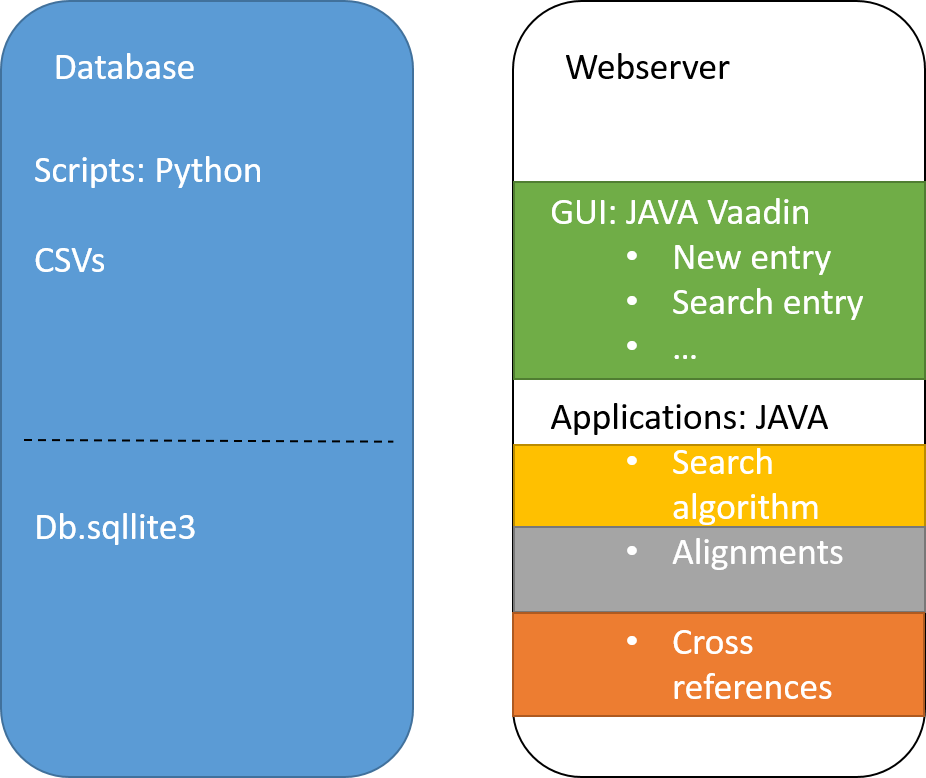
\includegraphics[width=\textwidth]{../img/Structure.png}
	\end{figure}

\section{ The Time-Plan}
Of course time is an important factor. Therefore, we started to organize a time plan for all of our ideas. This is of course the final plan. The setup of the DB should be finished in the first two weeks. It should be easy to set the DB up from the data we might get from our eventually partner lab. At the same time and through the whole project time, we want to work on the GUI. Because of adding of new functional modules also needs to happen in the GUI. But before starting blindly the GUI we want to design a general concept, allowing a reasonable integration. After the basics are finished we start to implement or integrate additional functions, like the search or the alignment algorithms. Time is the limiting factor of our project. Therefore, we want to add the modules one after another and if we cannot add all modules in time, this might be the case after the project.
  
	\begin{figure}[h]
		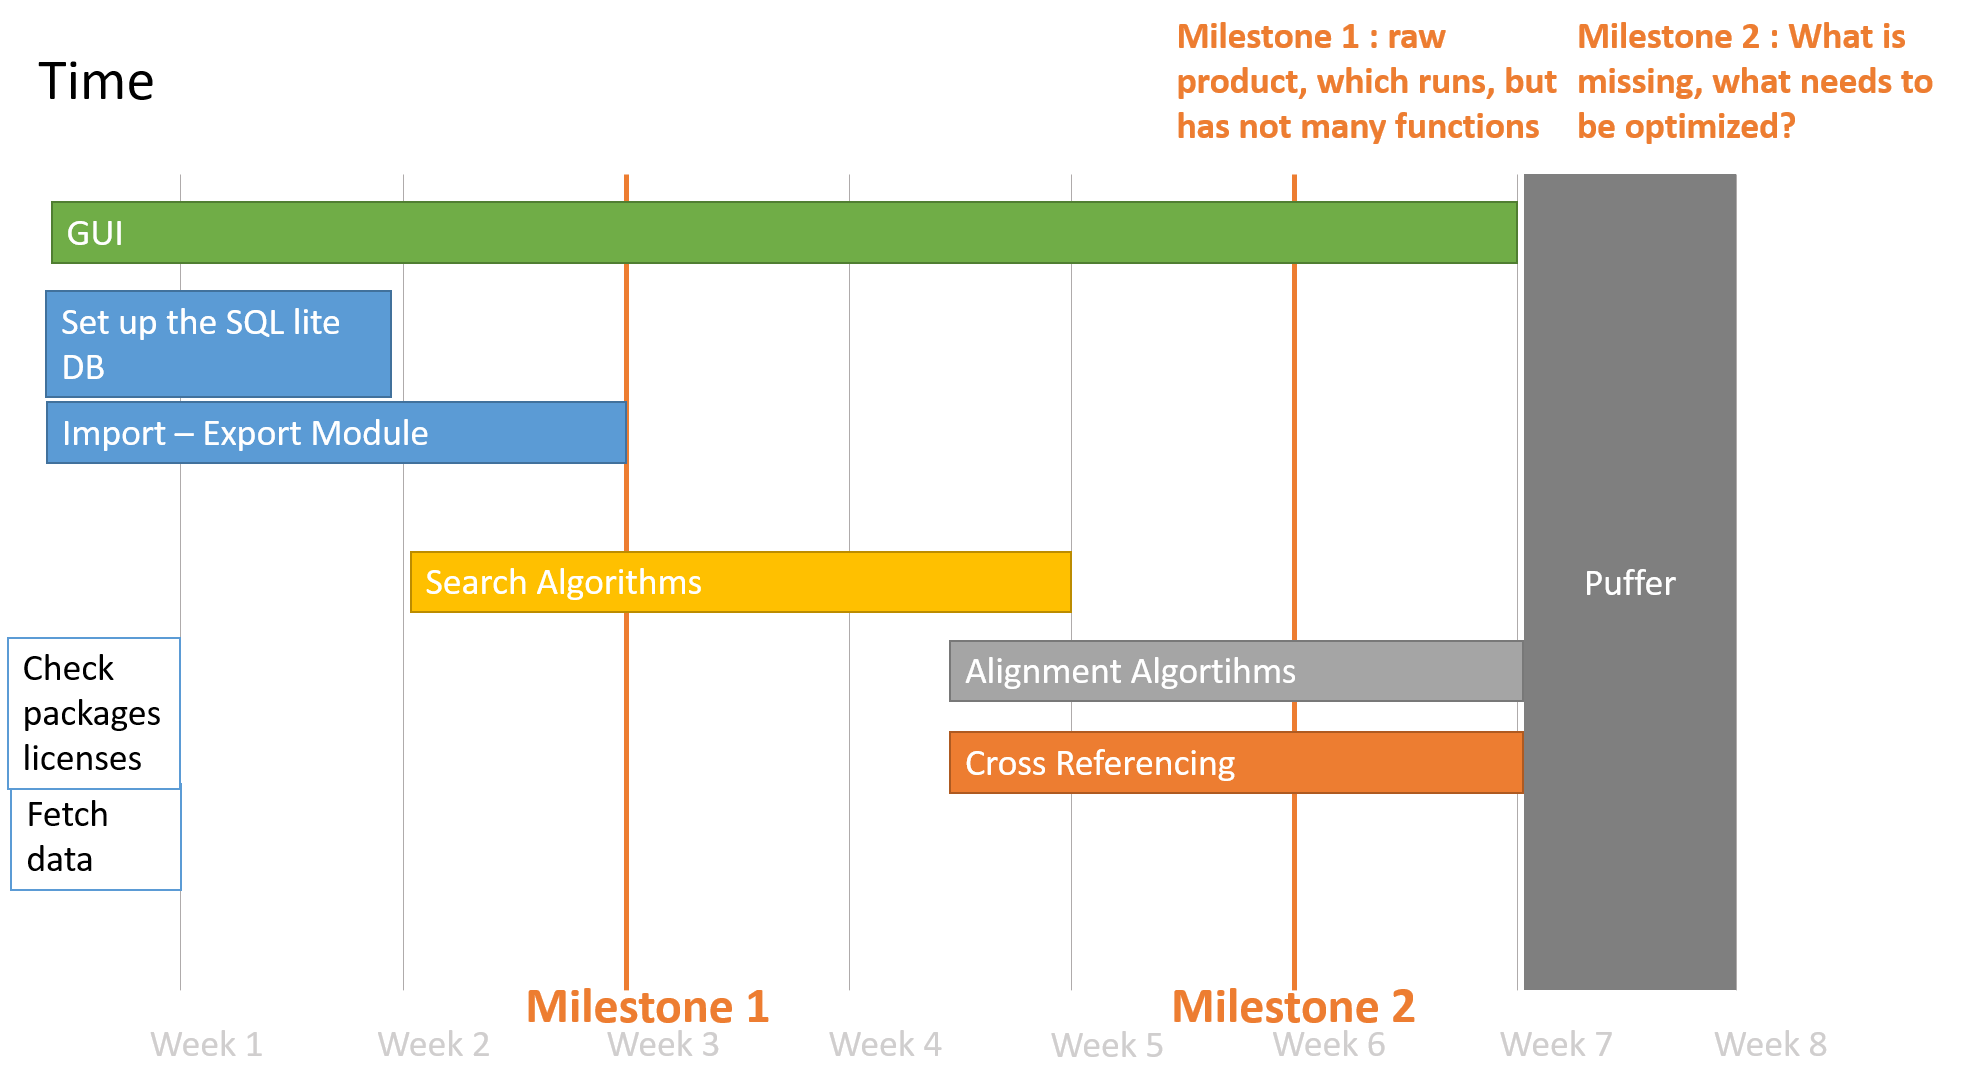
\includegraphics[width=\textwidth]{../img/Time.png}
	\end{figure}

\end{document}
